\chapter{联邦学习中的本地自适应差分隐私机制}

\label{ch3}

\section{引言}
与传统的集中式深度学习相比,联邦学习通过分布式训练在一定程度上缓解了隐私泄漏的问题。然而,许多研究表明,在训练过程中,本地设备与中央服务器之间的通信信道和传递的模型参数都有可能成为第三方窃取敏感信息的途径,联邦学习的框架仍然存在本地训练数据泄漏等隐私威胁\upcite{ref48}。深度学习技术可以“记忆”模型中的训练数据信息,在这种情况下,敌方一旦通过白盒推理攻击或者黑盒推理攻击访问模型,就可以推演出客户端本地的训练数据。

在第二章的基础知识中曾讲到,联邦学习模型的优化问题可以概括为ERM(经验风险最小化)问题\upcite{ref40}:
\begin{equation}\label{eq:ERM}
\arg \min _{\theta \in \mathcal{C}}\left(F(\theta):=\frac{1}{m} \sum_{i=1}^{m} F_{i}(\theta)\right)
\end{equation}

从隐私保护的角度讲,我们只要截断了从原始输入到输出,在其中加入一道隐私保护屏障,具体在哪一步截断则对应于不同的方法。差分隐私保护机器学习的方法具体有以下几种:
\begin{itemize}
	\item \textbf{输入扰动:} 输入扰动是在获取的训练数据上直接添加噪声,之后的模型训练和优化都是基于加躁后的训练数据\upcite{ref37}\upcite{ref38}\upcite{ref39}。
	\item \textbf{输出扰动:} 输出扰动沿袭了拉普拉斯机制最简单的思路,即考虑函数输出的敏感度来添加噪声,那么在ERM公式中我们只需要考虑argmin函数输出的敏感度,基于这个敏感度来添加拉普拉斯噪声即可得到一个简单的满足差分隐私的ERM方法\upcite{ref36}。
	\item \textbf{梯度扰动:} 梯度扰动是在执行最小化损失函数的过程中,设计满足差分隐私的算法。
	\item \textbf{目标扰动:} 目标扰动是在模型的目标函数中添加一个随机量,以使得最终模型的输出满足随机性。
\end{itemize}

基于输入的扰动和输出的扰动基本可以视为一个黑匣子模型,简单直接。但是这种添加噪声的方式无法对训练过程中数据的相互依赖性和输出有效性作出有用的、紧密的描述。在输入数据中加入过多的噪声,可能会影响模型训练的收敛性。在输出参数中加入过于保守的噪声,也就是根据最坏的攻击情况去添加噪声,可能会影响模型的实用性。

当前在深度学习模型中应用差分隐私的主流方案是在模型的梯度上添加噪声,方案的目标是在满足差分隐私的条件下,实现整体模型的最优可用性。Song等人\upcite{ref47}提出了一个$\left(\epsilon_{c}+\epsilon_{d}\right)$-差分隐私版本的随机梯度下降算法。在本地模型的每一次迭代过程中,对梯度添加高斯噪声,并通过差分隐私的组合性和隐私放大效果,得到完全隐私损失的上界。传统的联邦学习中使用差分隐私的主要流程如下所示:
\begin{itemize}
\item \textbf{本地计算:}
客户端 $\mathrm{i}$ 根据本地数据库 $\mathcal{D}_{\mathrm{i}}$ 和接受的服务器的全局模型 $\mathrm{w}_{\mathrm{G}}^{\mathrm{t}}$ 作为本地的参数,即 $\mathrm{w}_{\mathrm{i}}^{\mathrm{t}}=\mathrm{w}_{\mathrm{G}}^{\mathrm{t}}$, 采用梯度下降策略进行本地模型训练得到 $\mathrm{w}_{\mathrm{i}}^{\mathrm{t}+1} \quad(\mathrm{t}$ 表示当前通信回合) 。

\item \textbf{模型扰动:}
每个客户端产生一个随机噪音 $\mathrm{n},\mathrm{n}$ 是符合高斯分布的,使用 $\overline{\mathbf{w}_{\mathrm{i}}}^{\mathrm{t}+1}=\mathrm{w}_{\mathrm{i}}^{\mathrm{t}+1}+\mathrm{n}$ 扰动本地模型 (这里注意w是一个矩阵,n表示对矩阵的每一个元素添加噪音)。

\item \textbf{模型聚合:}
服务器使用参数聚合算法聚合从客户端收到的 $\overline{\mathrm{w}}_{\mathrm{i}} \mathrm{t}+1$ ,得到新的全局模型参数 $\mathrm{w}_{\mathrm{G}}^{\mathrm{t}+1}$, 也就是扰动过的模型参数。

\item \textbf{模型广播:}
服务器将新的模型参数广播给每个客户端。

\item \textbf{全局收敛:}
重复步骤(1)-(4)直至全局模型收敛。
\end{itemize}

与SGD 相比,差分隐私随机梯度下降 (DP-SGD) 严重降低了训练模型的效用。 如图所示,当差分隐私隐私提供的隐私强度增加时,MNIST数据集上逻辑回归的训练和验证的损失率迅速增加。由DP-SGD训练的卷积神经网络(CNN)的测试精度比MNIST 上的非差分隐私网络低得多。Goodfellow\upcite{ref64}提出了$\ell_{2}$范式梯度裁剪的方式以限制函数敏感度,并设计了“Moments Accountant”(MA)来计算更准确的隐私预算估计。

然而,在传统的基于差分隐私的联邦学习框架中,数据管理者倾向于给每个用户的数据以相同的隐私预算,同样的隐私预算忽略了用户之间的差异。有些用户希望有更好的隐私保护。而有些用户对某些数据的隐私不敏感。在这种情况下,由于联邦学习模型是分布式结构,从一个大数据库到许多小数据库,所以对于每个用户来说。他们只需要关心他们自己的隐私。他们可以设置不同的隐私预算方案,而不是传统的统一分配,然后在最坏的的情况下注入噪音。而基于梯度扰动的方法的问题在于它们的迭代性质会导致隐私预算的飙升。因此,当前的主要挑战是设计一种新型的满足差分隐私的扰动算法,既能保证模型的效用性,并且维持较高的计算效率。本文采用一种更加复杂的方法来分析训练过程中训练数据对模型输出的贡献比率,然后根据每一层神经网络对模型输出的贡献率,在梯度上自适应添加噪声,并在梯度下降的过程中采用拉普拉斯平滑机制保证模型的快速收敛。拉普拉斯平滑(Laplacian Smoothing,LS)可以看作是一种对高斯噪声注入的随机梯度进行后处理的去噪技术。

在本文中,我们认为中央参数服务器是半可信的(Honest but Curious, HbC),一个"诚实但好奇"的实体。也就是说,服务器将遵循与所有用户的协议。然而,通过利用通信信道访问用户梯度的便利,它也试图在训练过程中反推出关于客户端的额外的信息。出于这个原因,我们的提出的自适应加噪机制目的是保护发送到服务器的本地梯度不被推断出任何关于用户的本地训练样本信息,并且尽量维持原有模型的精度。为实现相同的效用保证,我们算法的梯度复杂度(即计算的随机梯度总数)为$O\left(n^{3 / 2}\right)$,比之前的最佳结果高出$\Theta\left(n^{1 / 2}\right)$。 之后我们在凸ERM和非凸ERM(逻辑回归和卷积神经网络)上进行实验,评估我们提出的方法,发现我们的方法不仅产生了在模型精度方面最接近非差分隐私的模型,而且还降低了计算成本。

总的来说,本章提出的隐私保护方案是基于本地客户端的本地数据维度,从以下三个方面展开研究:
\begin{enumerate}
\item [(1)] 通过在本地模型训练的梯度下降算法过程中针对不同层的贡献比自适应添加高斯噪声。
\item [(2)] 对于添加高斯噪声的梯度添加拉普拉斯平滑机制。
\item [(3)] 根据训练轮数和层间贡献率对梯度进行自适应裁剪。
\end{enumerate}

\section{相关理论}

\subsection{自适应噪声添加算法}
在第二章我们详细介绍了联邦学习的流程和神经网络的结构,每个用户在本地设备在私有数据集上进行训练,得到本地模型的输出。本地训练的流程如图\ref{fig:神经网络的前向传播和反向传播流程图}所示,神经网络中前向传播算法的第一步在输入层。我们使用前馈神经网络接收输入的$x$运行前向传播算法,得到预测值,然后通过反向传播算法不断调整参数使与预测值和真实值之间的误差降低。Bach等人提出了针对神经网络的逐层关联传播算法\upcite{ref65},它允许分解深度神经网络的预测值,我们利用该算法将神经网络的输出值按层进行分解,得到每层的属性值对于模型输出的贡献比,然后根据属性的贡献率,在梯度下降的过程中添加对应比的高斯噪声。

\begin{figure}[!hbt]
\centering
	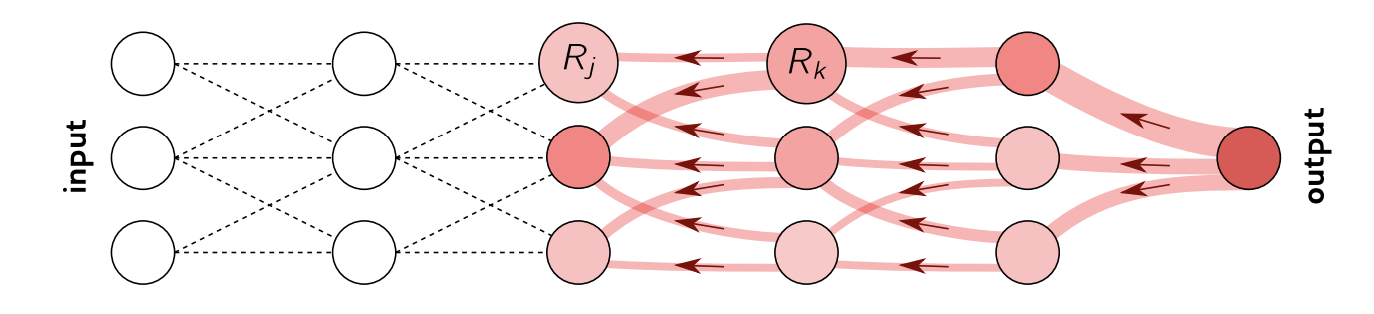
\includegraphics[scale=0.45]{fig2/C3/逐层关联传播算法}%联邦学习的系统架构
	\caption{神经网络的前向传播和反向传播流程图}
	\label{fig:神经网络的前向传播和反向传播流程图}	
\end{figure}

在逐层关联传播算法中,根据神经网络的结构自后向前计算归因值,也称为相关性分数。对于卷积神经网络等网络结构,从输出层开始根据反向传播算法计算归因分数,输出层的归因分数通常作为输出层的预激活值,在反向传播过程中,每一层的所有神经元的归因分数总和是恒定。

在卷积神经网络结构中,每个隐藏神经元的转化过程表示为$y=a(\mathbf{x} * \omega+b)$,其中$\mathbf{x}$代表输入向量,$y$是输出,$b$和$\omega$分别代表{}偏置项和权重矩阵。$a()$是一个激活函数,用于结合线性变换和非线性变换。

由于神经网络的结构,上一层的输出是下一层的输入,由此我们可以得出,原始的训练数据只被第一个隐藏层的线性变换所利用。直白地说,为了得到一个具有隐私保护的学习模型,我们可以在第一个隐藏层的数据中注入噪声。正如Phan等人\upcite{ref36}提到的,对于线性变换有一种传统的方法,即向原始数据注入具有相同隐私预算的噪声,但是这容易导致隐私预算增加,并且使原始数据失真过多。因此,本文提出一种自适应噪声添加算法,针对每个梯度计算其贡献值,根据属性对于模型输出的贡献率添加对应比例的高斯噪声。

令$C_{a_{i}}^{l_{k}}\left(x_{i}\right)$表示第$k$层的神经元 $a_{i}$,"$\leftarrow$"表示神经网络每一层之间的连接关系。"$l_{k} \leftarrow l_{k+1}$" 是指深度神经网络中第k层和第k+1层之间相邻层的连接关系。对于模型输出的贡献率,根据神经网络相邻层间的线形关系,那么神经元$a_{i}$的贡献率即为与之相邻的第$k+1$层的神经元的贡献率之和:
$$
C_{a_{i}}^{l_{k}}\left(x_{i}\right)=\sum_{a_{j} \in l_{k+1}} C_{a_{i} \leftarrow a_{j}}^{l_{k} \leftarrow l_{k+1}}\left(x_{i}\right)
$$

当第k层为输出层时,我们有:
\begin{equation}
C_{a_{i}}^{l_{k}}\left(x_{i}\right)=f\left(x_{i}, \omega_{i}^{r}\right)
\end{equation}

根据矩阵层之间的线性相关性,神经元$a_{i}$在第k层的贡献$C_{a_{i}}^{l_{k}}\left(x_{i}\right)$等于连接到神经元$a_{i}$的相邻层的贡献之和:
\begin{equation}\label{eq:层间传播1}
C_{a_{i}}^{l_{k}}\left(x_{i}\right)=\sum_{a_{j} \in l_{k+1}} C_{a_{i} \leftarrow a_{j}}^{l_{k} \leftarrow l_{k+1}}\left(x_{i}\right)
\end{equation}

因此,位于输出层的神经元$a_{j}$的贡献等于模型的输出。第k-1层的神经元$a_{j}$对于第k层的神经元的贡献$C_{a_{i} \leftarrow a_{j}}^{l_{k-1} \leftarrow l_{k}}\left(x_{i}\right)$等于:
\begin{equation}
C_{a_{i} \leftarrow a_{j}}^{l_{k-1} \leftarrow l_{k}}\left(x_{i}\right)=\left\{\begin{array}{cc}\frac{a_{i} w_{i, j}}{\sum_{a_{i} \in l_{k-1} a_{i} w_{i, j}}} C_{a_{j}}^{l_{k}}\left(x_{i}\right) & \sum_{a_{i} \in l_{k-1}} a_{i} w_{i, j} \neq 0 \\ \mu & \sum_{a_{i} \in l_{k-1}} a_{i} w_{i, j}=0\end{array}\right.
\end{equation}

其中$\mu$是一个无限接近于零,但大于零的数字。从上述公式中,我们可以认为每一层的贡献是相等的,而且贡献是逐层传递的。根据以上公式的推导,我们能得到神经网络模型中每一层以及每个神经元的贡献值。那么模型的输出可以表示为层神经元贡献值的累加:
$$
\begin{aligned}
\sum f\left(x_{i}, \omega_{i}^{r}\right) &=C_{a_{8}}^{l_{3}}\left(x_{i}\right)+C_{a_{9}}^{l_{3}}\left(x_{i}\right)\\
&+C_{a_{4}}^{l_{2}}\left(x_{i}\right)+C_{a_{5}}^{l_{2}}\left(x_{i}\right)+C_{a_{6}}^{l_{2}}\left(x_{i}\right)+C_{a_{7}}^{l_{2}}\left(x_{i}\right)\\
&+C_{a_{1}}^{l_{1}}\left(x_{i}\right)+C_{a_{2}}^{l_{1}}\left(x_{i}\right)+C_{a_{3}}^{l_{1}}\left(x_{i}\right)
\end{aligned}
$$

通过从数据元组中提取同一属性的贡献,我们可以计算出每个属性类对模型输出的平均贡献:
\begin{equation}\label{eq:属性添加自适应扰动}
C_{j}\left(x_{i}\right)=\frac{1}{n} \sum_{i=1}^{n} C_{x_{i, j}}\left(x_{i}\right), j \in[1, u]
\end{equation}

在原始的参数上计算神经网络中每个梯度对于模型输出的贡献后,按照公式\ref{eq:属性添加自适应扰动-拉普拉斯机制}采用高斯机制根据属性类的贡献率在属性值中注入噪音以保护原始的参数。
\begin{equation}\label{eq:属性添加自适应扰动-拉普拉斯机制}
\ddot{C}_{j}\left(x_{i}\right)=C_{j}\left(x_{i}\right)+\mathcal{N}\left(0, S_{f}^{2} \cdot \sigma^{2}\right), j \in[1, u]
\end{equation}
其中,函数的局部敏感度为$S_{f}=\frac{2 u}{|D|}$,$u,|D|$分别代表了属性和数据元组的最大数量。

然后,我们引入了两个调整参数$f$和$p$。其中,$f$代表一个阈值,用于决定属性对模型结果输出的归因分数是高还是低,其值由联邦学习中的本地用户自己定义,即贡献超过阈值$f$的梯度对输出的贡献更大,我们向所有这些梯度注入自适应拉普拉斯噪声。当归隐分数低于阈值$f$时,对这些梯度进行概率选择。也就是说,我们抛弃概率为$1-p$的原始数据,并对一些概率为$p$的梯度注入自适应拉普拉斯噪声。该公式如下:
\begin{equation}\label{eq:神经网络加噪}
\tilde{x}_{i, j}=\left\{\begin{array}{ll}
\ddot{x}_{i, j} & \beta \geq f \\
\bar{x}_{i, j} & \beta<f
\end{array}\right.
\end{equation}

其中$\beta$代表该层神经元的归因分数:$\beta=\frac{\left|\ddot{C}_{j}\right|}{\sum_{j=1}^{u}\left|\ddot{C}_{j}\right|}$,当$\beta<f$时,我们有:
\begin{equation}\label{eq:神经网络加噪2}
\bar{x}_{i, j}=\left\{\begin{array}{l}
\ddot{x}_{i, j} \text { with probability } p \\
x_{i, j} \text { with probability } 1-p
\end{array}\right.
\end{equation}

在此方案中,隐私预算$\epsilon_{l}$是根据各自的归因分数按比例分配给每个梯度:$\sigma$=$\sigma_{j}=\frac{u *\left|\ddot{C}_{j}\right|}{\sum_{j=1}^{u}\left|\ddot{C}_{j}\right|} * \sigma_{l}$,自适应高斯噪声按以下方式注入梯度中:
\begin{equation}\label{eq:神经网络加噪3}
x_{i, j}^{\prime}=x_{i, j}+\frac{1}{\left|D_{i}^{t}\right|}\mathcal{N}\left(0, S_{f}^{2} \cdot \sigma^{2}\right)
\end{equation}

在不失一般性的情况下,调整因子$f$和$p$的值与系统的准确性和隐私水平有关。即$f$越小,$p$越大,代表越高的隐私保护水平,模型准确性越低,反之亦然。算法ref{自适应高斯噪声算法}详细描述了自适应高斯噪声算法,我们将层间依赖算法于随机梯度下降算法相结合,关键的步骤包括:计算梯度以及归因分数,根据归因分数分配相应的隐私预算,在梯度上添加高斯噪声,最后进行梯度下降。

\begin{algorithm}[!htb]
	\caption{自适应高斯噪声算法}
	\label{自适应高斯噪声算法}
	\begin{algorithmic}[1]
		\footnotesize
		\STATE \textbf{输入:} 数据集 $\left\{x_{1}, \ldots, x_{N}\right\}$,损失函数$\mathcal{L}(\theta)=$ $\frac{1}{N} \sum_{i} \mathcal{L}\left(\theta, x_{i}\right)$,学习率$\eta_{t}$, 隐私预算$\sigma$, 批大小$L$
		\STATE 初始化:模型权重$\theta_{0}$
		\FOR{ $t \in[T]$}
			\STATE 以概率$L / N$随机采样一批数据集$L_{t}$
			\STATE 计算梯度\\$\mathbf{g}_{t}\left(x_{i}\right) \leftarrow \nabla_{\theta_{t}} \mathcal{L}\left(\theta_{t}, x_{i}\right)$
			\STATE 计算梯度的贡献率\\$\beta=\frac{\left|\ddot{C}_{j}\right|}{\sum_{j=1}^{u}\left|\ddot{C}_{j}\right|}$
			\STATE 根据贡献率分配相应的隐私预算\\$\sigma==\frac{u *\left|\ddot{C}_{j}\right|}{\sum_{j=1}^{u}\left|\ddot{C}_{j}\right|} * \sigma_{l}$
			\STATE 添加高斯噪声\\$\tilde{\mathbf{g}}_{t} \leftarrow \frac{1}{L} \sum_{i}\left(\overline{\mathbf{g}}_{t}\left(x_{i}\right)+\frac{1}{\left|D_{i}^{t}\right|}\mathcal{N}\left(0, S_{f}^{2} \cdot \sigma^{2}\right)\right)$
			\STATE 梯度下降\\$\theta_{t+1} \leftarrow \theta_{t}-\eta_{t} \tilde{\mathbf{g}}_{t}$
		\ENDFOR
		\STATE \textbf{输出:} $\theta_{t}$
	\end{algorithmic}
\end{algorithm}

\subsection{拉普拉斯平滑机制}
在本章的开头曾介绍了联邦学习中的ERM问题,它是模型训练的关键问题:在梯度下降的过程中,如何快速使ERM函数收敛,达到全局的最优点,使模型的输出值与真实值最接近,提高模型精度。因为我们已经在梯度中添加了高斯噪声,对模型的收敛速度也会产生影响,当ERM非凸时,可能导致函数无法达到全局最优点。因此,在本节中,我们提出了拉普拉斯平滑机制,针对加噪后的梯度,采用拉普拉斯平滑机制使随机梯度下降算法在非凸ERM和凸ERM的情况都能达到全局收敛。


\subsection{自适应梯度裁剪}
在传统的差分隐私随机梯度下降算法中,提供隐私保护的常用技术是限制函数的敏感度并添加与敏感度界限成比例的高斯噪声。为此,我们需要在每一轮SGD上限制梯度的敏感性。Abadi\upcite{ref65}等人提出通过梯度范数裁剪保证函数的敏感度有界。如果损失函数是可微的(如果不可微,则使用子梯度)和 Lipschitz 有界的,用Lipschitz 界限制梯度范数,并用它来推导出梯度的灵敏度。 如果损失函数导数作为输入的函数有界(例如,在逻辑回归的情况下,可以通过最大可能的输入范数来限制梯度范数),从而推导出梯度的灵敏度。 如果损失函数不像深度学习应用中那样具有已知的 Lipschitz 界,则很难推导出梯度范数的先验界。 在每次训练迭代中,可以使用经验值来获得梯度范数的近似界限,并在这个近似界限处裁剪梯度。 然而,经验值的可用性是一个强有力的假设,在没有经验值的情况下如何针对自适应添加的噪声裁剪梯度是一个难题。


\section{自适应差分隐私算法}
算法的主要思想是基于从先前更新中获得的信息迭代构建差分隐私梯度估计器$\mathbf{v}_{p}^{t}$。算法\ref{基于凸ERM的自适应差分隐私随机优化算法}详细描述了在本地客户端训练过程中,在SGD算法中添加自适应差分隐私,并使用差分隐私组合定理衡量所添加的噪声大小。首先,我们采用先验组合机制计算$eps_{iter}$和$\delta_{iter}$(算法第行)。每个客户端对训练数据进行采样,并计算他们的隐私预算$\delta_{u}$。如果$\delta_{u}>\delta$,用户将终止采样和训练,并且不上传其梯度信息(算法第11-13行)。然后,我们根据$\mathbf{v}^{t}=\nabla F_{\mathcal{B}_{t}}\left(\boldsymbol{\theta}^{t}\right)+(1-\gamma)\left(\mathbf{v}_{p}^{t-1}-\nabla F_{\mathcal{B}_{t}}\left(\boldsymbol{\theta}^{t-1}\right)\right)$等式不断的迭代更新$\mathbf{v}^{t}$,$\nabla F_{\mathcal{B}_{t}}\left(\boldsymbol{\theta}^{t}\right), \nabla F_{\mathcal{B}_{t}}\left(\boldsymbol{\theta}^{t-1}\right)$ 都表示小批量的随机梯度,$\mathbf{v}_{p}^{t-1}$是在最后一次迭代中计算得到的差分梯度估计器。$\gamma$表示动量参数,用于控制先验参数$\mathbf{v}_{p}^{t-1}-\nabla F_{\mathcal{B}_{t}}\left(\boldsymbol{\theta}^{t-1}\right)$的衰减率。这样的做法可以让早期的梯度对当前梯度的影响越来越小,如果没有衰减值,模型往往会震荡难以收敛,甚至发散。之后,对梯度进行范数裁剪(算法第17行),在更新后的权重系数$\mathbf{v}^{t}$上添加噪声矩阵为$\sigma_{2} \mathbf{I}_{d}$的高斯噪声$\mathbf{u}^{t}$,以使加噪后的梯度满足差分隐私。高斯随机向量的方差 $\sigma_{0}^{2}, \sigma^{2}$ 由我们基于RDP的分析确定,下文将仔细阐述。最后,服务器对用户上传的梯度进行聚合,并更新模型参数$w$。该算法有三个主要部分:带有动量的梯度估计,满足RDP的高斯噪声,自适应梯度裁剪。

\begin{algorithm}[!htb]
	\caption{差分隐私随机动量优化算法}
	\label{基于凸ERM的自适应差分隐私随机优化算法}{}
	\begin{algorithmic}[1]
		\footnotesize
		\STATE \textbf{输入:} 预估迭代次数$T$,学习率$\alpha$,梯度裁剪阈值$C$,目标损失函数$l$,隐私参数$\epsilon, \delta$,
		\STATE \textbf{输出:} 模型梯度
		\STATE 初始化模型权重$\boldsymbol{\theta}^{0}$
		\STATE 初始化动量梯度估计:$\mathbf{v}_{p}^{0}=\mathbf{v}^{0}+\mathbf{u}^{0}$
		\WHILE{$\exists \delta_{u}<\delta$}
			\STATE $n$=0
			\STATE $grad$=0
			\STATE 计算$eps_{iter}$,$\delta_{iter}$
			\FOR {each $u \in$ Users}
				\STATE 计算$\delta_{u}$
				\IF{$\delta_{u}>\delta$}
					\STATE continue
				\ENDIF
				\STATE 从客户端数据集中随机采样
				\STATE $g t_{u}=\nabla l(\boldsymbol{\theta}^{0}, x)$
				\STATE 自适应梯度裁剪
				\STATE $\boldsymbol{\theta}^{t+1}=\boldsymbol{\theta}^{t}-\eta_{t} \mathbf{v}_{p}^{t}$,其中$\eta_{t}=\min \left\{\zeta /\left(n_{0} L\left\|\mathbf{v}_{p}^{t}\right\|_{2}\right), 1 /\left(2 n_{0} L\right)\right\}$
				\STATE 添加高斯噪声
				\STATE $\mathbf{v}^{t+1}=\nabla F_{\mathcal{B}_{t+1}}\left(\boldsymbol{\theta}^{t+1}\right)+(1-\gamma)\left(\mathbf{v}_{p}^{t}-\nabla F_{\mathcal{B}_{t+1}}\left(\boldsymbol{\theta}^{t}\right)\right)$,其中噪声满足$\mathbf{u}^{t+1} \sim N\left(0, \sigma^{2} \mathbf{I}_{d}\right)$
				\STATE 更新动量梯度估计
				\STATE $\mathbf{v}_{p}^{t+1}=\mathbf{v}^{t+1}+\mathbf{u}^{t+1}$
				\STATE $n$++
			\ENDFOR
			\STATE $\boldsymbol{\theta}^{0}=\boldsymbol{\theta}^{0}-\alpha * g r a d / n$
		\ENDWHILE
	\end{algorithmic}
\end{algorithm}

在算法\ref{基于凸ERM的自适应差分隐私随机优化算法}中,假使其中的每个优化函数都满足$G$-Lipschitz,并且有$L$-Lipschitz的梯度。给定总迭代次数$T$,动量参数$\alpha$和一阶驻点的准确率$\zeta$。对于任意的$\delta>0$和隐私预算$\epsilon$。$b_{0}$和$b$表示批大小,当噪声参数$\sigma_{0}^{2}=14 T G^{2} \alpha /\left(\beta n^{2} \epsilon\right)$和$\sigma^{2}=14 T((1-$ $\left.\gamma) \zeta / n_{0}+\gamma G\right)^{2} \alpha /\left(\beta n^{2} \epsilon\right)$时,基于凸ERM的自适应差分私有随机优化算法满足$(\epsilon, \delta)$-差分隐私。

我们的算法要求每个分量函数$f_{i}$是$G$-Lipschitz,并且具有$L$-Lipschitz的梯度。该梯度将用于推导底层查询函数(即算法 \ref{基于凸ERM的自适应差分隐私随机优化算法}中的梯度动量$\mathbf{v}^{t}$)的敏感性,从而确定高斯噪声。同时,我们采用梯度裁剪技术保证在每轮迭代过程中满足$\left\|\nabla f_{i}\left(\boldsymbol{\theta}^{t}\right)\right\|_{2} \leq C_{1}$ and $\left\|\nabla f_{i}\left(\boldsymbol{\theta}^{t}\right)-\nabla f_{i}\left(\boldsymbol{\theta}^{t-1}\right)\right\|_{2} \leq C_{2}$,其中$C_{1}$和$C_{2}$由本地用户预先定义。梯度动量$\mathbf{v}^{t}$的敏感度上界为$2\left((1-\gamma) C_{2}+\gamma C_{1}\right) / b$。

在模型的每一轮迭代过程中,算法将计算添加了高斯噪声的梯度$\mathbf{v}^{t+1}=\nabla F_{\mathcal{B}_{t+1}}\left(\boldsymbol{\theta}^{t+1}\right)+(1-\gamma)\left(\mathbf{v}_{p}^{t}-\nabla F_{\mathcal{B}_{t+1}}\left(\boldsymbol{\theta}^{t}\right)\right)$,其中噪声满足$\mathbf{u}^{t+1} \sim N\left(0, \sigma^{2} \mathbf{I}_{d}\right)$。对梯度注入的噪声量为$\frac{1}{\left|D_{i}^{t}\right|} \operatorname{Lap}\left(\frac{G S_{l}}{\epsilon_{j}}\right)$,决定于用户个体对于梯度 $g$ 在二范数下的最大全局敏感度, 即$\delta$ 。由于梯度的大小没有一个先验的界限, 我们采用二范数的固定值对每个梯度进行裁剪。

用户上传的梯度向量可以改写为$g t_{u}=g t_{u} / \max \left(1, \frac{\left\|g t_{u}\right\|}{C}\right)$, 其中 $C$是裁剪阈值。对于梯度的裁剪能保证梯度值小于设定的阈值$\mathrm{i}$。 也就是当 $\|g\| \leq C$ ,$g$ 保持不变;当$\|g\|>C$ 时, 它会按照裁剪比例缩小为 $C_{\circ}$。

但是如果裁剪阈值$C$ 的值如果太小,那么裁剪后的噪声会较小,算法添加的噪声较小时可能会破坏梯度估计的无偏性;可是如果不对梯度进行裁剪,大量的噪声添加到每个梯度会导致模型的可用性大大降低。在模型训练前期,梯度所包含的数据信息更多,因此可以对应添加更多的拉普拉斯噪声,使用较大的$C$ 的值,使得梯度裁剪后的模型偏差更小;而在模型训练后期,梯度所包含的数据信息相对较小了,如果还使用相同的$C$ ,会引入很多不必要的噪声。

因此我们根据训练轮数和层间贡献率动态调整梯度裁剪阈值$C$:在每次迭代中,该算法使用方差为$S_{f} \sigma$的高斯机制来计算噪声梯度$g t_{u}^{\prime}=g t_{u}+\frac{1}{\left|D_{i}^{t}\right|} \operatorname{Lap}\left(\frac{G S_{l}}{\epsilon_{j}}\right)$。噪声$S_{f} \sigma$的大小取决于一个个体在$l_{2}$规范下对$g$的最大影响,即$\delta$。由于对梯度的大小没有先验的约束,我们以$l_{2}$规范对每个梯度进行裁剪。因此,梯度向量$g$被$g t_{u}=g t_{u} / \max \left(1, \frac{\left\|g t_{u}\right\|}{C}\right)$取代,以达到裁剪阈值$C$。这种裁剪保证了如果$|g t_{u}\| \leq C$,那么$g t_{u}$将被保留,而如果$|g\|>C$,它将被裁减为梯度范数$C$。

在本章接下来的两节,我们将给出基于凸ERM的自适应差分隐私随机优化算法关于隐私保证和模型效用性的证明,并与前人的方案进行对比。

\section{隐私性证明}
根据算法\ref{基于凸ERM的自适应差分隐私随机优化算法},在第t轮迭代过程采用的算法为$\mathcal{M}_{t}$,由0~t轮的高斯噪声组成:$\mathcal{G}_{0}, \ldots, \mathcal{G}_{t}$,其中$\mathcal{G}_{0}=\nabla F_{\mathcal{B}_{0}}\left(\boldsymbol{\theta}^{0}\right)+\mathbf{u}^{0}$,$\mathcal{G}_{t}=\nabla F_{\mathcal{B}_{t}}\left(\boldsymbol{\theta}^{t}\right)-$ $(1-\gamma) \nabla F_{\mathcal{B}_{t}}\left(\boldsymbol{\theta}^{t-1}\right)+\mathbf{u}^{t}$。因此本节证明$\mathcal{M}_{t}$是满足差分隐私的。假设模型的训练集为$S$,$S^{\prime}$表示与$S$第$i^{\prime}$个数据记录不同的相邻数据集。

对于算法$\mathcal{M}_{t}$给出严格的隐私证明存在两个难点:1.算法中的子采样机制$\left\{\mathcal{G}_{i}\right\}_{i=0}^{T-1}$;2.当$t>0$,如何控制$\mathcal{G}_{t}$的敏感度。第一个难点可以通过我们的子采样定理\ref{高斯机制实现RDP算法}的隐私放大来解决,这为我们提供了隐私保证的紧密封闭形式。对于第二个难点,我们可以通过使用自适应步长,使用更少量的随机噪声来实现差分隐私。

根据算法\ref{基于凸ERM的自适应差分隐私随机优化算法},$\mathcal{G}_{t}$表示在从训练集$S$中均匀采样的样本集$\mathcal{B}_{t}$上应用高斯机制$\widetilde{\mathcal{G}}_{t}$:
$$
\widetilde{\mathcal{G}}_{t}=\left\{\begin{array}{ll}
\frac{1}{b} \sum_{i=1}^{n} \nabla f_{i}\left(\boldsymbol{\theta}^{0}\right)+\mathbf{u}^{0}, & t=0 \\
\frac{1}{b} \sum_{i=1}^{n}\left(\nabla f_{i}\left(\boldsymbol{\theta}^{t}\right)-\phi \nabla f_{i}\left(\boldsymbol{\theta}^{t-1}\right)\right)+\mathbf{u}^{t}, & t>0
\end{array}\right.
$$
其中,$\phi=1-\gamma$。对于$\widetilde{\mathcal{G}}_{0}$中的$\widetilde{\mathbf{q}}_{0}=\sum_{i=1}^{n} \nabla f_{i}\left(\boldsymbol{\theta}^{0}\right) / b_{0}$,$\Delta\left(\widetilde{\mathbf{q}}_{0}\right)$的敏感度由下式决定:
$$
\left\|\widetilde{\mathbf{q}}_{0}(S)-\widetilde{\mathbf{q}}_{0}\left(S^{\prime}\right)\right\|_{2} \leq \frac{1}{b}\left\|\nabla f_{i}\left(\boldsymbol{\theta}^{0}\right)-\nabla f_{i^{\prime}}\left(\boldsymbol{\theta}^{0}\right)\right\|_{2} \leq \frac{2 G}{b_{0}}
$$
该式的最后一个不等子式由算法\ref{基于凸ERM的自适应差分隐私随机优化算法}中的每个子函数的$G$-Lipschitz决定,对于$\widetilde{\mathcal{G}}_{t}$中的$\widetilde{\mathbf{q}}_{t}=$ $\sum_{i=1}^{n} \nabla f_{i}\left(\boldsymbol{\theta}^{t}\right) / b-(1-\gamma) \sum_{i=1}^{n} \nabla f_{i}\left(\boldsymbol{\theta}^{t-1}\right) / b$,当$t>0$时,函数$\Delta\left(\widetilde{\mathbf{q}}_{t}\right)=\| \widetilde{\mathbf{q}}_{t}(S)-$ $\widetilde{\mathbf{q}}_{t}\left(S^{\prime}\right) \|_{2}$的敏感度由下式决定:
$$
\frac{1-\gamma}{b}\left\|\nabla f_{i}\left(\boldsymbol{\theta}^{t}\right)-\nabla f_{i}\left(\boldsymbol{\theta}^{t-1}\right)+\nabla f_{i^{\prime}}\left(\boldsymbol{\theta}^{t}\right)-\nabla f_{i^{\prime}}\left(\boldsymbol{\theta}^{t-1}\right)\right\|_{2}+\frac{\gamma}{b}\left\|\nabla f_{i}\left(\boldsymbol{\theta}^{t}\right)-\nabla f_{i^{\prime}}\left(\boldsymbol{\theta}^{t}\right)\right\|_{2}
$$
因此,可以推理出:
$$
\begin{aligned}
\left\|\mathbf{q}_{t}(S)-\mathbf{q}_{t}\left(S^{\prime}\right)\right\|_{2} & \leq \frac{2 L(1-\gamma)}{b}\left\|\boldsymbol{\theta}^{t}-\boldsymbol{\theta}^{t-1}\right\|_{2}+\frac{2 \gamma G}{b} \\
&=\frac{2 L(1-\gamma)}{b} \eta_{t-1}\left\|\mathbf{v}_{p}^{t-1}\right\|_{2}+\frac{2 \gamma G}{b} \\
& \leq \frac{2(1-\gamma) \zeta}{n_{0} b}+\frac{2 \gamma G}{b}
\end{aligned}
$$

该式的第一个不等子式由$L$-Lipschitz的连续梯度和每个子函数的$G$-Lipschitz决定。最后一个不等子式由算法中选择的自适应步长$\eta_{t}=\min \left\{\zeta /\left(n_{0} L\left\|\mathbf{v}_{p}^{t}\right\|_{2}\right), 1 /\left(2 n_{0} L\right)\right\}$决定。$\eta_{t}$自适应步长是控制函数$\widetilde{\mathbf{q}}_{t}$敏感度有界的关键,如果我们选择一个固定的步长$\eta_{t}=1 /(2 L)$,函数$\widetilde{\mathbf{q}}_{t}$敏感度会按照$O\left(G^{2} / b\right)$的顺序。这将导致算法需要添加更大的随机噪声来实现差分隐私,从而降低了模型的效用。

根据定理\ref{高斯机制实现RDP算法},如果添加高斯噪声的参数满足$\sigma_{0}^{2}=14 T \alpha G^{2} /\left(\beta n^{2} \epsilon\right)$和$\sigma^{2}=$ $14 T \alpha\left((1-\gamma) \zeta / n_{0}+\gamma G\right)^{2} /\left(\beta n^{2} \epsilon\right)$,高斯机制$\widetilde{\mathcal{G}}_{t}$满足$\left(\alpha, \beta \epsilon n^{2} /\left(7 b_{0}^{2} T\right)\right)$-RDP,子采样造成的隐私放大效应显示 $\mathcal{G}_{t}$满足$(\alpha, \beta \epsilon / T)$-RDP。因此结合高斯机制和子采样机制的算法$\mathcal{G}_{t}$ 满足$(\alpha, \beta \epsilon / T)$-RDP。根据RDP的组合性质,在$T^{\prime}$轮迭代之后,算法\ref{基于凸ERM的自适应差分隐私随机优化算法}满足$\alpha=\log (1 / \delta) /((1-\beta) \epsilon)+1$-RDP。根据定理\ref{RDP向DP的转换},当$\alpha=\log (1 / \delta) /((1-\beta) \epsilon)+1$时,算法\ref{基于凸ERM的自适应差分隐私随机优化算法}满足$\left(T^{\prime} \epsilon / T, \delta\right)$-差分隐私。

\section{模型效用分析}
根据 $\widetilde{\boldsymbol{\theta}}$的定义,可以得到:
$$
\mathbb{E}\|\nabla F(\widetilde{\boldsymbol{\theta}})\|_{2}=\frac{1}{T} \sum_{t=0}^{T-1} \mathbb{E}\left\|\nabla F\left(\boldsymbol{\theta}^{t}\right)\right\|_{2} \leq \frac{1}{T} \sum_{t=0}^{T-1} \mathbb{E}\left\|\mathbf{v}_{p}^{t}\right\|_{2}+\frac{1}{T} \sum_{t=0}^{T-1} \mathbb{E}\left\|\nabla F\left(\boldsymbol{\theta}^{t}\right)-\mathbf{v}_{p}^{t}\right\|_{2}
$$
其中期望值覆盖算法的所有随机性。对于算法\ref{基于凸ERM的自适应差分隐私随机优化算法}建立严格的效用保证的关键挑战是如何在自适应步长$\eta_{t}$和梯度$\mathbf{v}_{p}^{t}$上的随机噪声$\mathbf{u}^{t}$
推导出$\sum_{t=0}^{T-1} \mathbb{E}\left\|\mathbf{v}_{p}^{t}\right\|_{2} / T$ and $\sum_{t=0}^{T-1} \mathbb{E}\left\|\nabla F\left(\boldsymbol{\theta}^{t}\right)-\mathbf{v}_{p}^{t}\right\|_{2} / T$的严格上界。

首先,考虑到自适应步长$\eta_{t}$,推导出$\sum_{t=0}^{T-1} \mathbb{E}\left\|\mathbf{v}_{p}^{t}\right\|_{2} / T$ 的上界:
$$
\frac{4 n_{0} L D_{F}}{T \zeta}+\frac{1}{T \zeta} \sum_{t=0}^{T-1} \mathbb{E}\left\|\nabla F\left(\boldsymbol{\theta}^{t}\right)-\mathbf{v}_{p}^{t}\right\|_{2}^{2}+2 \zeta
$$
其中,$D_{F}=F\left(\boldsymbol{\theta}^{0}\right)-F\left(\boldsymbol{\theta}^{*}\right)$。然后,可以推导出项$\sum_{t=0}^{T-1} \mathbb{E} \| \mathbf{v}_{p}^{t}-$ $\nabla F\left(\boldsymbol{\theta}^{t}\right) \|_{2}^{2} / T$的上界:
$$
\frac{2(1-\gamma)^{2} \zeta^{2}}{n_{0}^{2} \gamma b}+\frac{2 \gamma G^{2}}{b}+\frac{G^{2}}{T \gamma b_{0}}+\frac{T d \sigma^{2}+d \sigma_{0}^{2}}{T \gamma}
$$
该多项式的第一项由自适应步长$\eta_{t}$决定,最后一项由在梯度$\mathbf{v}_{p}^{t}$上的随机噪声$\mathbf{u}^{t}$决定。该边界的最后一项由$d \sigma^{2} / \gamma$决定,从而验证了通过自适应步长能有效控制$\mathbf{v}^{t}$ 的敏感度,添加噪声的参数 $\sigma^{2}$越小,即能保证模型的效用越高。

最后,结合上述给出的两个上界,可以得到:
$$
\mathbb{E}\|\nabla F(\widetilde{\boldsymbol{\theta}})\|_{2} \leq C_{1} \zeta+C_{2} \frac{\sqrt{L D_{F} d \log (1 / \delta)} G}{n \epsilon \zeta}
$$
通过控制 $\zeta$可以得到$\zeta=\left(L D_{F} d \log (1 / \delta)\right)^{1 / 4}\left(C_{2} G\right)^{1 / 2} /\left(C_{1} n \epsilon\right)^{1 / 2}$。因此,$\mathbb{E}\|\nabla F(\widetilde{\boldsymbol{\theta}})\|_{2} \leq C_{3} \zeta$,其中$C_{1}, C_{2}, C_{3}$是常数。

\section{隐私预算分析}
本章所提出的自适应差分隐私保护方案是通过在随机梯度下降算法上添加自适应的拉普拉斯扰动,保护数据的隐私性。在上一节我们已经证明了此算法满足$\left(\epsilon_{c}+\epsilon_{l}\right)$差分隐私,那另外一个非常重要的问题就是评估在训练过程中添加噪声所累积的隐私预算成本。在本节中,我们提出动量组合的概念,去计算算法迭代过程中添加噪声所累积的隐私预算成本。

根据差分隐私的并串行组合定理,被查询n次的数据的隐私预算将增加n倍。因此,我们希望查询次数越少越好,至少要有一个界限。在实验环境中,我们可以通过几次尝试确定一个相对理想的迭代次数,然后在每次迭代中平均分配隐私预算。然而,在实践中很难选择迭代的数量,因为任何尝试都会增加额外的隐私风险。当数量太小时,会发生预拟合,导致性能不佳;如果数量太大,注入的噪声会过大,这将影响模型的准确性。另一种尝试是使用等比例递增的注入噪声序列,这样无论我们有多少次迭代,我们都能找到有限的隐私预算\upcite{ref32}。

根据上文提出的差分隐私的并串行组合定理,我们设计了一个动量组合定理:
\begin{theorem}[动量组合定理]\label{动量组合定理}
假使存在算法$M_{i}$满足$\left(\varepsilon_{i}, \delta_{i}\right)$-差分隐私,那么对于$M_{[k]}=\left(M_{1}, M_{2}, \ldots, M_{k}\right)$,有$M_{[k]}$也是满足$(\varepsilon, \delta)$-差分隐私的,其中
$$
\delta=\sum_{i=1}^{k} B(i, k, p)\left[\Phi\left(\frac{H \sqrt{i}}{2 \sigma}-\frac{\varepsilon \sigma}{H \sqrt{i}}\right)-e^{\varepsilon} \Phi\left(-\frac{H \sqrt{i}}{2 \sigma}-\frac{\varepsilon \sigma}{H \sqrt{i}}\right)\right]
$$
\end{theorem}

我们采用朴素贝叶斯机制计算$\delta$可以得到:
\begin{equation}\label{eq:朴素贝叶斯}
\delta=\sum_{i=1}^{k} B(i, k, p)\left[\operatorname{Pr}\left[L_{d, d^{\prime}} * i>\varepsilon\right]-e^{\varepsilon} \operatorname{Pr}\left[L_{d^{\prime}, d} * i<-\varepsilon\right]\right]
\end{equation}

在此情况下,隐私损失变量$L_{M, d, d^{\prime}}$和$L_{M, d^{\prime}, d}$同时满足$N(\eta, 2 \eta)$分布,并且$\eta=$ $H^{2} / 2 \sigma^{2}$。因此可以采用动量组合定理这样表达隐私预算损失:
\begin{equation}\label{eq:隐私预算计算1}
\begin{aligned}
& \operatorname{Pr}\left[L_{d, d^{\prime}} * i>\varepsilon\right]=\operatorname{Pr}[N(\eta i, 2 \eta i)>\varepsilon] \\
=& \operatorname{Pr}\left[N(0,1)>\frac{-\eta i+\varepsilon}{\sqrt{2 \eta i}}\right]=\operatorname{Pr}\left[N(0,1)<\frac{\eta i-\varepsilon}{\sqrt{2 \eta i}}\right] \\
=& \operatorname{Pr}\left[N(0,1)<\sqrt{\frac{\eta i}{2}}-\frac{\varepsilon \sigma}{\sqrt{2 \eta i}}\right]=\Phi\left(\frac{H \sqrt{i}}{2 \sigma}-\frac{\varepsilon \sigma}{H \sqrt{i}}\right)
\end{aligned}
\end{equation}

然后,可以计算得到隐私预算:
\begin{equation}\label{eq:隐私预算计算2}
\delta=\sum_{i=1}^{k} B(i, k, p)\left[\Phi\left(\frac{H \sqrt{i}}{2 \sigma}-\frac{\varepsilon \sigma}{H \sqrt{i}}\right)-e^{\varepsilon} \Phi\left(-\frac{H \sqrt{i}}{2 \sigma}-\frac{\varepsilon \sigma}{H \sqrt{i}}\right)\right]
\end{equation}

因为随着算法迭代次数$T$的增加,$\Phi\left(\frac{H \sqrt{T}}{2 \sigma}-\frac{\varepsilon \sigma}{H \sqrt{T}}\right)-e^{\varepsilon} \Phi\left(-\frac{H \sqrt{T}}{2 \sigma}-\frac{\varepsilon \sigma}{H \sqrt{T}}\right)$也在增加,因此可以计算得到:

\begin{equation}\label{eq:隐私预算计算3}
\begin{aligned}
& \sum_{i=1}^{T} B(i, T, p)\left[\operatorname{Pr}\left[L_{d, d^{\prime}} * i>\varepsilon\right]-e^{\varepsilon} \operatorname{Pr}\left[L_{d^{\prime}, d} * i<-\varepsilon\right]\right] \\
\leq & \sum_{i=1}^{T} B(i, T, p)\left[\operatorname{Pr}\left[L_{d, d^{\prime}} * T>\varepsilon\right]-e^{\varepsilon} \operatorname{Pr}\left[L_{d^{\prime}, d} * T<-\varepsilon\right]\right] \\
\leq & \operatorname{Pr}\left[L_{d, d^{\prime}} * T>\varepsilon\right]-e^{\varepsilon} \operatorname{Pr}\left[L_{d^{\prime}, d} * T<-\varepsilon\right]
\end{aligned}
\end{equation}

当隐私预算$\delta$相同时,$\sigma_{1} \leq \sigma_{2} \leq \sigma_{3}$。替换$\sigma=\alpha H \sqrt{T} / \sqrt{2 \epsilon}$,则有
\begin{equation}\label{eq:隐私预算计算4}
\Phi(\sqrt{\epsilon / 2}(1 / \alpha-\alpha))-e^{\varepsilon} \Phi(-\sqrt{\epsilon / 2}(1 / \alpha+\alpha)) \leq \delta
\end{equation}

因此,$\sigma_{1} \leq \sigma_{3}=O(\sqrt{T})$。与之前的工作相比,我们的隐私预算能够在相同的迭代次数$T$,更低的上紧界,达到满足$\left(\epsilon_{c}+\epsilon_{l}\right)$的差分隐私。


\section{本章总结}


